\documentclass[11pt,a4paper]{article}
\usepackage[utf8]{inputenc}
\usepackage[T1]{fontenc}
\usepackage[spanish]{babel}
\usepackage{geometry}
\geometry{top=2.0cm, bottom=2.2cm, left=2.0cm, right=2.0cm}
\usepackage{graphicx}
\usepackage{subcaption}
\usepackage{booktabs}
\usepackage{longtable}
\usepackage{array}
\usepackage{tabularx}
\usepackage{cite}
\usepackage{fancyhdr}
\usepackage{lastpage}
\usepackage{hyperref}

\hypersetup{
	colorlinks=true,
	linkcolor=black,
	citecolor=blue,
	urlcolor=blue
}

% --- ENCABEZADO Y PIE DE PÁGINA PERSONALIZADO ---
\pagestyle{fancy}
\fancyhf{}
\fancyhead[L]{\small \textbf{UTEQ -- ISR-401}}
\fancyhead[R]{\small \textbf{Especificación de Requisitos: Microsoft Teams}}
\fancyfoot[C]{\small Página \thepage\ de \pageref{LastPage}}
\renewcommand{\headrulewidth}{0.4pt}
\renewcommand{\footrulewidth}{0.4pt}

\begin{document}
	
	% --- PORTADA / DATOS GENERALES ---
	\begin{center}
		{\Large \textbf{Norma IEEE 29148 y Tipos de Requisitos Aplicados a un Sistema Colaborativo}} \\[0.15cm]
		{\large \textbf{Trabajo Individual de Ingeniería de Requerimientos}} \\[0.25cm]
		\textbf{Estudiante:} Freddy David Rochina Rochina \\[0.05cm]
		\textbf{Asignatura:} Ingeniería de Requerimientos (ISR-401) -- Paralelo B \\[0.05cm]
		\textbf{Institución:} Universidad Técnica Estatal de Quevedo (UTEQ) \\[0.05cm]
		\textbf{Docente:} Gleiston Cicerón Guerrero Ulloa, PhD \quad \textbf{Fecha límite:} 7 de noviembre de 2026
	\end{center}
	\hrule
	\vspace{0.25cm}
	
	% --- SECCIÓN 1 ---
	\section*{\textbf{1. Delimitación y Contexto Operativo del Sistema Seleccionado}}
	El sistema objeto de estudio es \textbf{Microsoft Teams}, una plataforma tecnológica de colaboración empresarial y educativa que centraliza la comunicación sincrónica y asincrónica mediante canales de texto, llamadas de voz, videoconferencias y repositorios de archivos compartidos. Los usuarios directos comprenden a la comunidad académica de la UTEQ, específicamente estudiantes y docentes que interactúan de forma remota para gestionar asignaturas, entregar tareas y coordinar actividades formativas. El entorno operativo se fundamenta en arquitecturas de red basadas en la nube e interfaces multiplataforma (aplicación de escritorio, móvil y cliente web). El presente análisis se circunscribe a las funciones de gestión de equipos, canales, mensajería y calendario institucional. Las características operativas y los límites funcionales se apoyan en la documentación técnica de la plataforma y en los estándares normativos vigentes \cite{iso29148_2018, iso25010_2023}.
	
	\begin{figure}[htbp]
		\centering
		\begin{subfigure}[b]{0.31\textwidth}
			\centering
			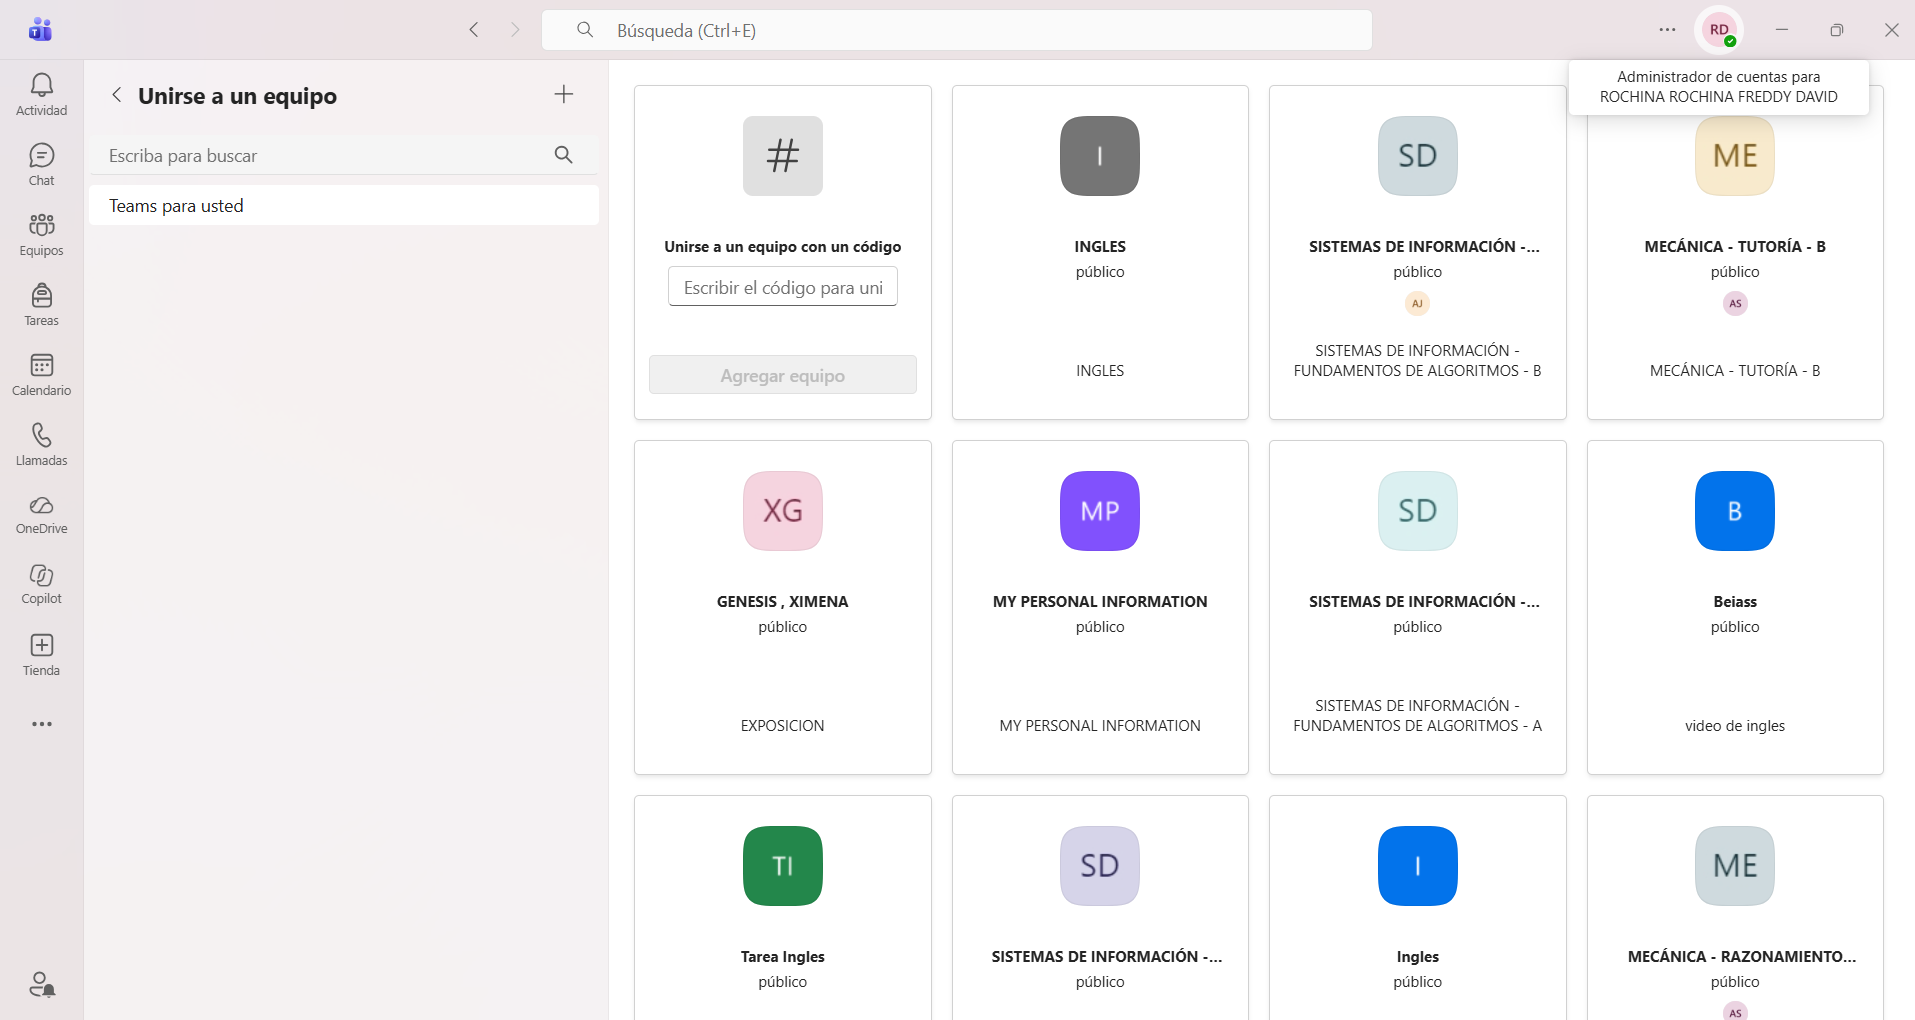
\includegraphics[width=\textwidth]{figuras/captura1.png}
			\caption{E1 -- Equipos (RF01)}
		\end{subfigure}
		\hfill
		\begin{subfigure}[b]{0.31\textwidth}
			\centering
			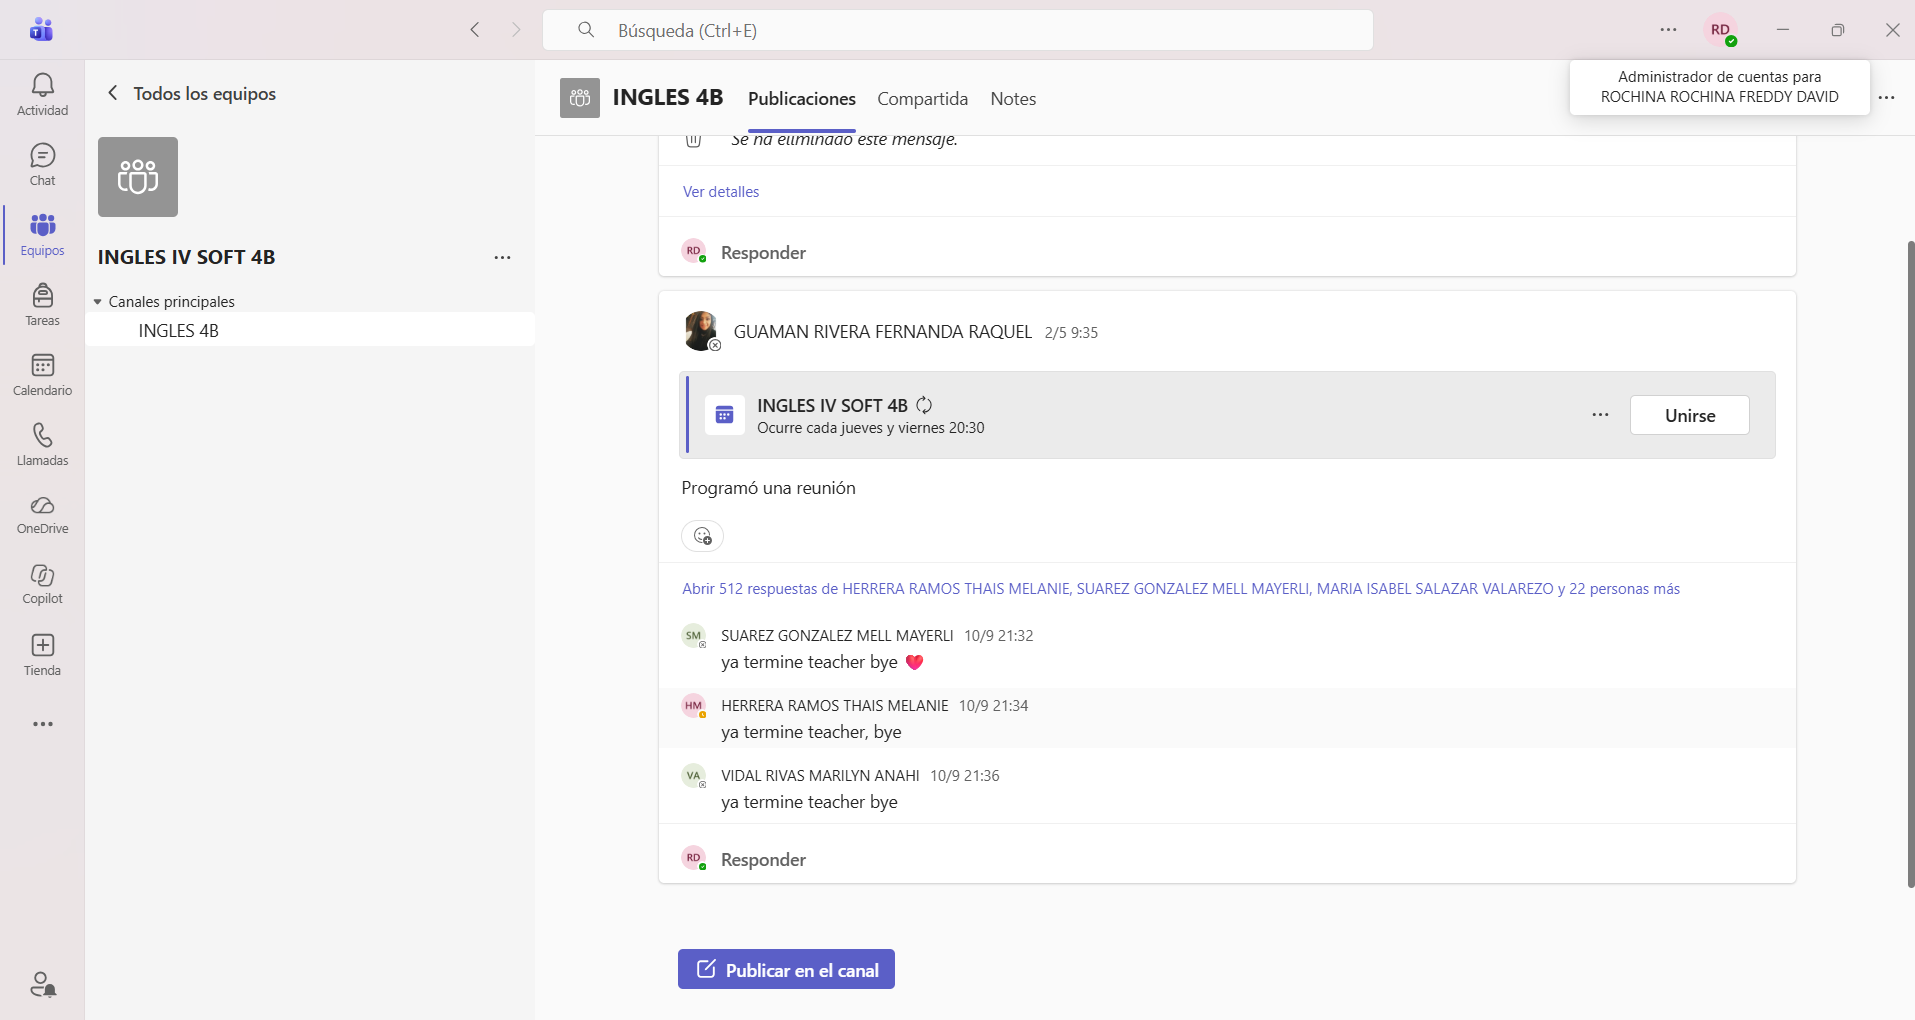
\includegraphics[width=\textwidth]{figuras/captura2.png}
			\caption{E2 -- Chat y Canales (RF03, RH01)}
		\end{subfigure}
		\hfill
		\begin{subfigure}[b]{0.31\textwidth}
			\centering
			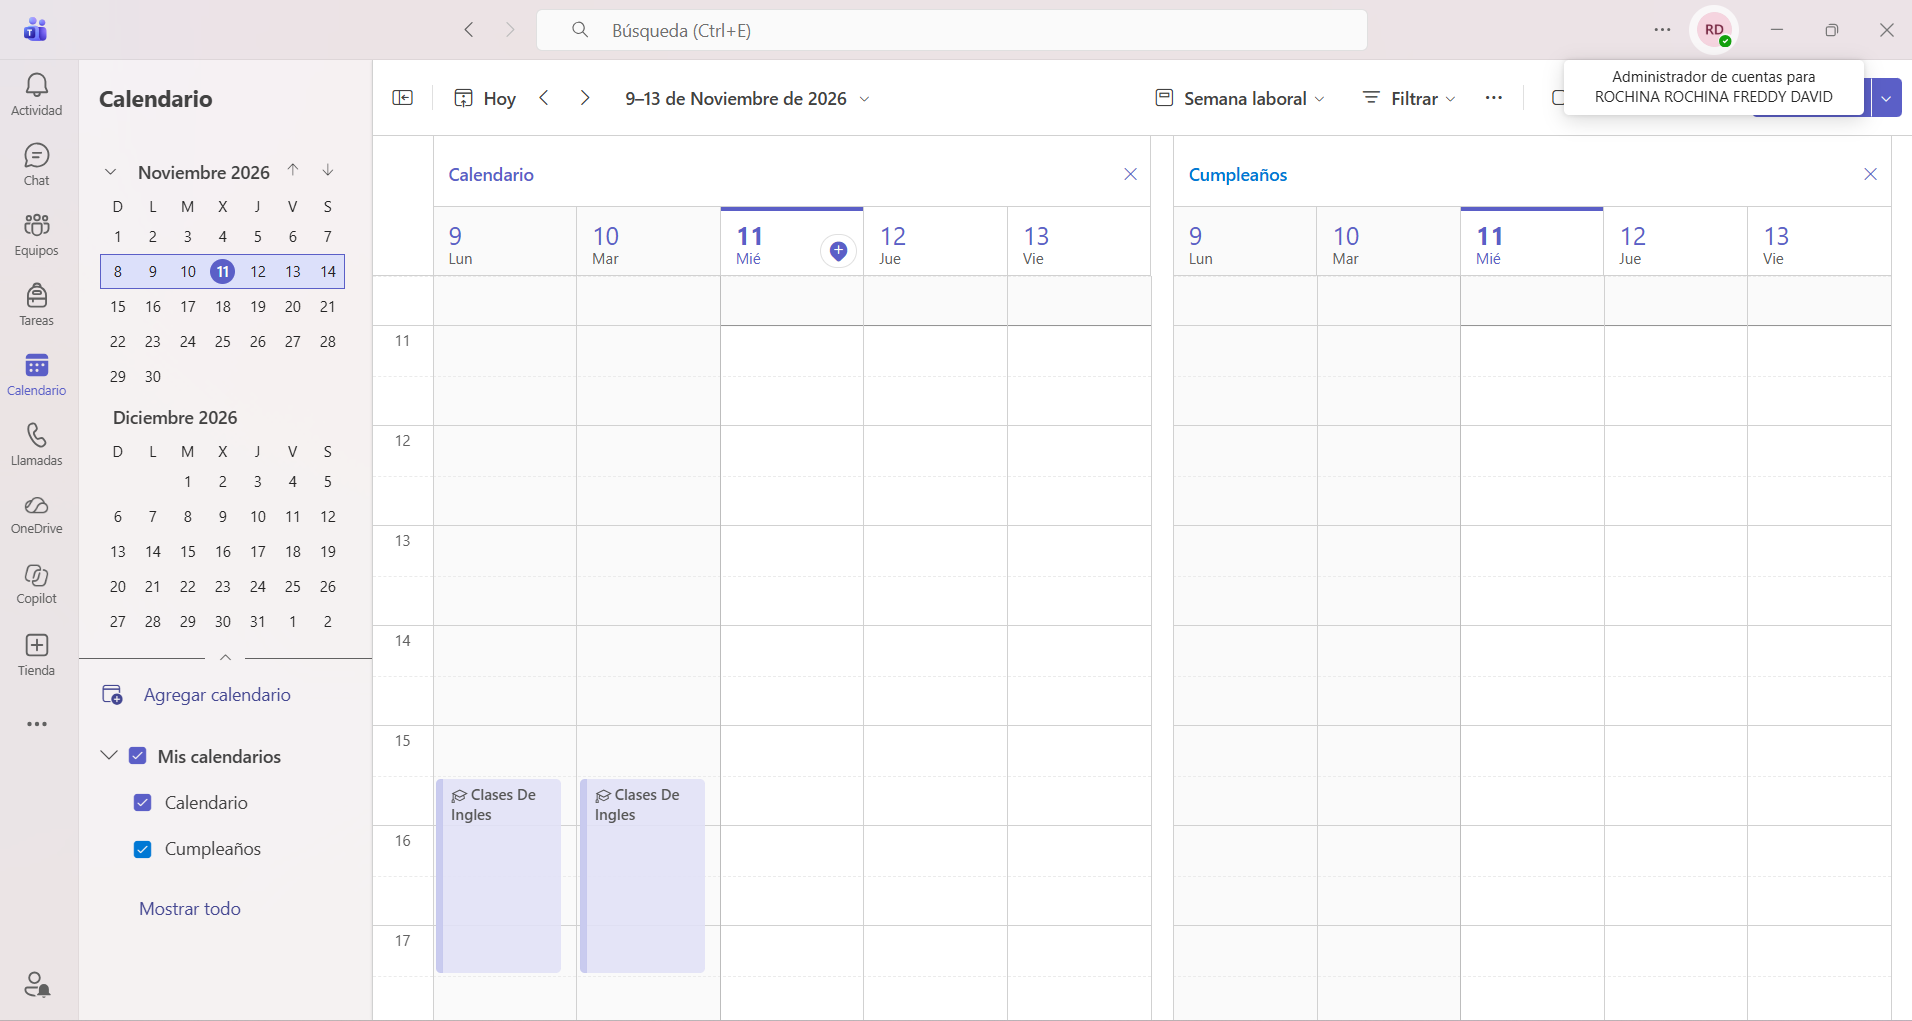
\includegraphics[width=\textwidth]{figuras/captura3.png}
			\caption{E3 -- Calendario (RF06)}
		\end{subfigure}
		\caption{\textbf{Figura 1:} Ubicación de tres capturas \textit{propias} que sustentan los requisitos del sistema. La exposición de datos sensibles y correos institucionales ha sido anonimizada conforme a las directrices de privacidad.}
		\label{fig:capturas_teams}
	\end{figure}
	
	La figura 1 identifica la evidencia de interfaz necesaria para sustentar parte de la matriz de requisitos; la exposición de datos personales, correos y nombres de usuarios reales se encuentra anonimizada para cumplir con los protocolos de seguridad y buenas prácticas en la gestión de repositorios académicos.
	
	% --- SECCIÓN 2 (SIN SALTO DE PÁGINA FORZADO) ---
	\section*{\textbf{2. Fundamentación Teórica y Análisis Crítico de la Norma ISO/IEC/IEEE 29148:2018}}
	La norma ISO/IEC/IEEE 29148:2018 establece los lineamientos para la ingeniería de requisitos dentro del ciclo de vida del software \cite{iso29148_2018}. El análisis exegético de sus cláusulas principales permite estructurar adecuadamente las especificaciones técnicas:
	
	\subsection*{\textbf{2.1 Estructura sintáctica del requisito bien formado}}
	Conforme a la cláusula 5.2.4, un requisito bien formado debe expresar una capacidad o restricción comprobable mediante una estructura gramatical clara que evite ambigüedades de diseño \cite{iso29148_2018}. En Microsoft Teams, esto implica especificar el comportamiento observable del sistema ante una acción del usuario en lugar de describir detalles de implementación interna o algoritmos de base de datos \cite{pohl2025}.
	
	\subsection*{\textbf{2.2 Propiedades normativas del requisito individual}}
	La cláusula 5.2.5 demanda el cumplimiento de nueve propiedades esenciales: ser necesario, apropiado, no ambiguo, completo, singular, factible, verificable, correcto y conforme \cite{iso29148_2018}. Esto garantiza que cada sentencia represente una única obligación técnica medible y libre de juicios subjetivos \cite{swebok2024}.
	
	\subsection*{\textbf{2.3 Criterios de calidad colectiva y control del lenguaje técnico}}
	Las cláusulas 5.2.6 y 5.2.7 abordan la consistencia del conjunto de requisitos y prohíben taxativamente el uso de términos ambiguos (como ``rápido'', ``adecuado'' o ``fácil'') que impidan la validación objetiva en la fase de pruebas \cite{iso29148_2018}. Asimismo, la cláusula 5.2.8 y el modelo ISO/IEC 25010:2023 diferencian con precisión los requerimientos funcionales de los atributos de calidad del producto \cite{iso25010_2023, pressman2020}.
	
	% --- SECCIÓN 3 (FLUYE CONTINUAMENTE SIN HUECOS) ---
	\section*{\textbf{3. Vocabulario Técnico Normalizado (Glosario Cláusula 3)}}
	A partir de la cláusula 3 de la norma, se definen diez términos clave adaptados analíticamente a Microsoft Teams:
	
	\begin{longtable}{p{3.0cm} p{5.0cm} p{6.8cm}}
		\caption{Glosario técnico normalizado aplicado al sistema Microsoft Teams.} \\
		\toprule
		\textbf{Término (Cláusula)} & \textbf{Definición conceptual} & \textbf{Aplicación práctica en Microsoft Teams} \\
		\midrule
		\endfirsthead
		\multicolumn{3}{c}{\tablename\ \thetable\ -- \textit{Continuación de la página anterior}} \\
		\toprule
		\textbf{Término (Cláusula)} & \textbf{Definición conceptual} & \textbf{Aplicación práctica en Microsoft Teams} \\
		\midrule
		\endhead
		\bottomrule
		\endfoot
		Restricción (3.1.7) & Condición limitante del diseño o implementación \cite{iso29148_2018}. & Compatibilidad del cliente con sistemas operativos específicos. \\
		Requisito (3.1.19) & Necesidad documentada convertida en obligación \cite{iso29148_2018}. & El sistema deberá permitir la creación de un nuevo equipo de trabajo. \\
		Elicitación (3.1.20) & Proceso sistemático de recolección de necesidades \cite{iso29148_2018}. & Identificar las funciones que requiere un docente al impartir clases. \\
		Ingeniería (3.1.21) & Disciplina integral de gestión y análisis de requerimientos \cite{iso29148_2018}. & Estudiar los permisos de acceso y roles en los canales de clase. \\
		Gestión (3.1.22) & Control de cambios y trazabilidad del ciclo de vida \cite{iso29148_2018}. & Versionar el requisito RF03 ante cambios en la interfaz de chat. \\
		Trazabilidad (3.1.23) & Relación biunívoca entre necesidad, requisito y prueba \cite{iso29148_2018}. & Vincular el requisito RF04 con la pestaña de archivos y su test. \\
		Matriz (3.1.24) & Registro estructurado de dependencias y fuentes \cite{iso29148_2018}. & Asociar el requisito RC02 a la norma ISO 25010 y a pruebas de seguridad. \\
		Validación (3.1.25) & Comprobación de que el sistema satisface al usuario \cite{iso29148_2018}. & Verificar con los estudiantes si la alerta de mención `@` es útil. \\
		Verificación (3.1.26) & Inspección de la correcta formulación sintáctica \cite{iso29148_2018}. & Revisar que los enunciados cumplan las nueve propiedades de la norma. \\
		Parte interesada (3.1.28) & Actor con legítimo interés en el funcionamiento \cite{iso29148_2018}. & Estudiante que entrega deberes y docente que evalúa en la plataforma. \\
		\bottomrule
	\end{longtable}
	
	% --- SECCIÓN 4 (SIN SALTO FORZADO PARA LLENAR EL ESPACIO) ---
	\section*{\textbf{4. Formulación, Tipificación y Métricas de los Requisitos del Sistema}}
	Se definen quince requisitos técnicos utilizando la nomenclatura: RF (Funcional), RI (Interfaz Externa), RP (Proceso), RU (Usabilidad en uso), RH (Factores Humanos) y RC (Calidad de Producto bajo ISO/IEC 25010:2023) \cite{iso25010_2023}.
	
	\begin{longtable}{p{0.8cm} p{4.3cm} p{1.6cm} p{2.3cm} p{2.2cm} p{2.8cm}}
		\caption{Matriz de especificación y clasificación de 15 requisitos para Microsoft Teams.} \\
		\toprule
		\textbf{ID} & \textbf{Enunciado verificable} & \textbf{Tipo} & \textbf{ISO 25010:2023} & \textbf{Métrica} & \textbf{Criterio de aceptación} \\
		\midrule
		\endfirsthead
		\multicolumn{6}{c}{\tablename\ \thetable\ -- \textit{Continuación de la página anterior}} \\
		\toprule
		\textbf{ID} & \textbf{Enunciado verificable} & \textbf{Tipo} & \textbf{ISO 25010:2023} & \textbf{Métrica} & \textbf{Criterio de aceptación} \\
		\midrule
		\endhead
		\bottomrule
		\endfoot
		RF01 & Permitir la creación de un equipo institucional autenticado \cite{iso29148_2018}. & Funcional & -- & Registro de datos & Credenciales válidas crean el equipo; inválidas deniegan acceso. \\
		RF02 & Aceptar correos institucionales para agregar miembros \cite{iso29148_2018}. & Funcional & -- & Validación de entrada & Correo válido añade al usuario; formato erróneo genera error. \\
		RF03 & Mostrar la vista previa del mensaje antes de publicarlo \cite{iso29148_2018}. & Funcional & -- & Visualización previa & El texto aparece en el cuadro de edición antes de confirmar. \\
		RF04 & Presentar el listado de documentos en la pestaña Archivos \cite{iso29148_2018}. & Funcional & -- & Directorio accesible & El repositorio muestra los archivos subidos al canal. \\
		RF05 & Generar alerta visual y sonora ante menciones con `@` \cite{iso29148_2018}. & Funcional & -- & Notificación activa & La mención emite aviso destacado en el cliente. \\
		RF06 & Programar reuniones indicando fecha, hora de inicio y fin \cite{iso29148_2018}. & Funcional & -- & Evento agendado & La reunión se sincroniza en el calendario integrado. \\
		RF07 & Compartir la pantalla activa con los participantes de la sala \cite{iso29148_2018}. & Funcional & -- & Transmisión de video & La ventana seleccionada se visualiza correctamente en red. \\
		RI01 & Sincronizar eventos programados con calendarios externos \cite{iso29148_2018}. & Interfaz ext. & -- & Conectividad API & El calendario externo recibe la invitación del evento. \\
		RI02 & Enlazar conexiones directas a salas de videoconferencia \cite{iso29148_2018}. & Interfaz ext. & -- & Redirección válida & El enlace institucional conduce a la sala correspondiente. \\
		RP01 & Registrar pruebas de conectividad previas a actualizaciones \cite{iso29148_2018}. & Proceso & -- & Informe técnico & Versión desplegada con acta de pruebas firmada. \\
		RU01 & Localizar archivos en un tiempo menor o igual a 60 s \cite{iso29148_2018}. & Usabilidad & -- & Tiempo de tarea & 8 de 10 usuarios nuevos ubican el archivo en el plazo. \\
		RH01 & Mostrar advertencia previa al eliminar un equipo de trabajo \cite{iso29148_2018}. & Factores hum. & -- & Aviso visual & Alerta visible antes de confirmar la eliminación de datos. \\
		RC01 & Completar el historial de chat en $\le 2.0\text{ s}$ (50 sesiones) \cite{iso25010_2023}. & Calidad & Desempeño: temporal & P95 (segundos) & En 200 consultas instrumentadas, $\text{P95} \le 2,0\text{ s}$. \\
		RC02 & Impedir el acceso a equipos privados sin credenciales \cite{iso25010_2023}. & Calidad & Seguridad: confidencialidad & Intentos bloqueados & 0 accesos exitosos en 30 ensayos negativos controlados. \\
		RC03 & Garantizar una disponibilidad mensual $\ge 99,9\%$ \cite{iso25010_2023}. & Calidad & Fiabilidad: disponibilidad & Porcentaje uptime & Medición de servicio continuo superior a $99,9\%$. \\
		RC04 & Permitir la edición del mensaje antes del envío definitivo \cite{iso25010_2023}. & Calidad & Interacción: errores & Corrección activa & 20 de 20 ensayos permiten modificar el texto redactado. \\
		RC05 & Evitar duplicidad de mensajes ante retransmisiones \cite{iso25010_2023}. & Calidad & Seguridad: integridad & Mensajes duplicados & 0 duplicados en 20 simulaciones de red autorizadas. \\
		\bottomrule
	\end{longtable}
	
	% --- SECCIÓN 5 ---
	\section*{\textbf{5. Análisis de Trazabilidad y Evidencias de Campo}}
	La trazabilidad metodológica vincula las funciones observadas en las capturas de pantalla con los fundamentos normativos y las guías de soporte oficial \cite{iso29148_2018, sommerville2016}. Las figuras 1 (E1, E2, E3) sustentan la interfaz analizada; sin embargo, se aclara que los requerimientos de calidad (RC01 a RC05) constituyen propuestas académicas sujetas a verificación mediante pruebas de caja negra en entornos controlados, protegiendo en todo momento la confidencialidad de los datos institucionales \cite{lehtola2005}.
	
	% --- SECCIÓN 6 ---
	\section*{\textbf{6. Matriz de Autoevaluación y Refinamiento Léxico}}
	Se evaluaron los requerimientos frente a las nueve propiedades individuales (N, A, U, C, S, F, V, Co, Cf) y los criterios de lenguaje estipulados en la norma \cite{iso29148_2018}.
	
	\begin{longtable}{p{1.2cm} p{3.2cm} p{1.6cm} p{7.0cm}}
		\caption{Inspección de calidad individual y control de ambigüedades léxicas.} \\
		\toprule
		\textbf{ID} & \textbf{Propiedades (NAUCSFV Co Cf)} & \textbf{Lenguaje} & \textbf{Evaluación analítica} \\
		\midrule
		\endfirsthead
		\multicolumn{4}{c}{\tablename\ \thetable\ -- \textit{Continuación de la página anterior}} \\
		\toprule
		\textbf{ID} & \textbf{Propiedades (NAUCSFV Co Cf)} & \textbf{Lenguaje} & \textbf{Evaluación analítica} \\
		\midrule
		\endhead
		\bottomrule
		\endfoot
		RF01--RF07 & PRRRRPR PR & Correcto & Enunciados singulares y verificables con cuenta de prueba \cite{iso29148_2018}. \\
		RI01--RI02 & PRRRRPR PR & Correcto & Delimitación estricta de interfaces externas \cite{iso29148_2018}. \\
		RP01--RU01 & PRRRRPR PR & Correcto & Procesos y métricas de usabilidad planteados formalmente \cite{iso29148_2018}. \\
		RH01 & PRRRRPR PR & Correcto & Advertencias de factores humanos claramente establecidas \cite{iso29148_2018}. \\
		RC01--RC05 & PRRRRPR PR & Correcto & Umbrales de calidad cuantificados sin términos vagos \cite{iso25010_2023}. \\
		\bottomrule
	\end{longtable}
	
	La corrección de enunciados defectuosos se detalla a continuación para demostrar la eliminación de ambigüedades:
	
	\begin{longtable}{p{1.0cm} p{4.6cm} p{5.2cm} p{3.2cm}}
		\caption{Control de versiones: corrección de enunciados ambiguos.} \\
		\toprule
		\textbf{ID} & \textbf{Versión inicial (con defectos)} & \textbf{Versión corregida (normativa)} & \textbf{Defecto superado} \\
		\midrule
		\endfirsthead
		\multicolumn{4}{c}{\tablename\ \thetable\ -- \textit{Continuación de la página anterior}} \\
		\toprule
		\textbf{ID} & \textbf{Versión inicial (con defectos)} & \textbf{Versión corregida (normativa)} & \textbf{Defecto superado} \\
		\midrule
		\endhead
		\bottomrule
		\endfoot
		RF02 & «El sistema debe permitir enviar mensajes fácilmente». & «Aceptar correos institucionales para agregar miembros al equipo». & Subjetividad léxica \cite{iso29148_2018}. \\
		RF03 & «Teams mostrará toda la información importante». & «Mostrar la vista previa del mensaje antes de publicar». & Término vago «importante» \cite{iso29148_2018}. \\
		RH01 & «Se mostrará un aviso claro si es posible». & «Mostrar advertencia previa al eliminar un equipo». & Cláusula evasiva \cite{iso29148_2018}. \\
		RC01 & «El historial de chat cargará muy rápido». & «Completar el historial de chat en $\le 2.0\text{ s}$ (50 sesiones)». & Adverbio impreciso \cite{iso25010_2023}. \\
		\bottomrule
	\end{longtable}
	
	% --- SECCIÓN 7 ---
	\section*{\textbf{7. Reflexión Crítica sobre los Retos de la Ingeniería de Requisitos}}
	El desarrollo de esta actividad pone de manifiesto que la mayor dificultad en la ingeniería de requisitos no radica en la enumeración de funciones visibles de un sistema, sino en la correcta cuantificación y modelado de los atributos de calidad \cite{iso25010_2023}. La transición de un enunciado intuitivo a una métrica verificable bajo la norma ISO/IEC/IEEE 29148:2018 exige rigor analítico y la eliminación absoluta de subjetividades \cite{iso29148_2018}. Esta práctica es vital para prevenir discrepancias contractuales y técnicas entre desarrolladores y usuarios finales.
	
	% --- SECCIÓN 8 ---
	\section*{\textbf{8. Declaración Explícita de Uso de Inteligencia Artificial}}
	De conformidad con las políticas de integridad académica de la UTEQ:
	\begin{itemize}
		\item \textbf{Herramienta:} Asistente de Inteligencia Artificial (Google Gemini).
		\item \textbf{Propósito:} Apoyo en la estructuración sintáctica del documento en LaTeX y verificación del formato bibliográfico IEEE.
		\item \textbf{Verificación:} En el desarrollo de la presente actividad académica se emplearon herramientas de asistencia digital e inteligencia artificial de manera consultiva, exclusivamente como soporte para la consulta de sintaxis en entornos de compilación LaTeX y la revisión ortotipográfica del texto. Todas las decisiones metodológicas, la selección de Microsoft Teams como caso de estudio, la formulación analítica de los requisitos, el desarrollo de las matrices lo cual se desarrollo de manera manual  para la culminacion de este trabajo.
	\end{itemize}
	
	% --- SECCIÓN 9 ---
	\section*{\textbf{9. Referencias Bibliográficas}}
	\bibliographystyle{IEEEtran}
	\bibliography{referencias}
	
\end{document}